\documentclass{article}
\usepackage[utf8]{inputenc}
\usepackage[T1]{fontenc}
\usepackage{amsmath,amssymb}
\usepackage{xcolor}
\usepackage{graphicx}
\usepackage{tikz}
\usetikzlibrary{arrows,positioning}
\usepackage{listings}
\usepackage{hyperref}
\usepackage{fancyhdr}   % For custom headers/footers
\usepackage{parskip}     % Adds spacing between paragraphs
\hypersetup{
    colorlinks=true,
    linkcolor=blue,
    urlcolor=blue,
    citecolor=blue
}

\title{Anti-Fragile Scientific Knowledge Blockchain: Breaking Free From Scientism}
\author{Bruno Coelho}
\date{2025}

% === Header/Footer Customization ===
\pagestyle{fancy}
\fancyhf{} % clear all header and footer fields

\lfoot{\textbf{Version 0.2}}     % Left footer
\cfoot{}                         % Center footer (you could put page numbers here)
\rfoot{\thepage}                % Right footer - page number

% Optional: line at the top
\renewcommand{\headrulewidth}{0pt}
% Optional: line at the bottom
\renewcommand{\footrulewidth}{0.1pt}

\begin{document}
\maketitle

\begin{abstract}
Scientific truth should be determined by the weight and structure of evidence—especially refutation (\emph{via negativa}) over time—not by popularity, reputation, or consensus. Yet modern science has increasingly become entangled with \textbf{Scientism}: a belief system that treats science as an authority to be obeyed, rather than a method to be tested.

The Antifragile Science Blockchain (ASB) is a direct response to this epistemic corruption. It is both a protocol and a platform: the protocol defines how scientific claims are evaluated through a falsifiability-first framework, and the platform provides the open infrastructure where researchers, reviewers, and adversarial testers interact with and evolve the knowledge graph. In ASB, failed claims strengthen the system. Refutations are not buried; they are rewarded.

This paper articulates the philosophical foundations of ASB, drawing on Karl Popper's principle of falsifiability and Nassim Nicholas Taleb's concepts of \emph{antifragility} and \emph{skin in the game}. We argue that refutation (“not all swans are white”) provides far greater epistemic value than confirmation, especially in complex, non-linear systems where false confidence leads to systemic harm.

The ASB protocol implements an antifragile scientific system—one that grows stronger with every attempt to find faults, both in the system itself and in the body of knowledge it holds. By contrasting this model with the fragile, consensus-driven methods promoted by Scientism—where dissent is suppressed, negative results ignored, and incentives warped—we expose the hidden vulnerabilities in the current scientific establishment.

Through an open, censorship-resistant platform and a citation-weighting algorithm based on Evidence Fragility Score (EFS), ASB realigns science with adversarial testing, transparency of incentives, and the permanent recording of failed hypotheses. The result is not a system that fears being broken—but one that welcomes it (or even needs it!).
\end{abstract}

\section*{Preamble}
\textit{GitHub Repository:} \url{https://github.com/w1ldrabb1t/antiscichain}\\

\textit{This paper was initially authored by a single contributor. However, the use of “we” throughout reflects its collaborative intent. The document is published under the GPLv3 license in a public GitHub repository and welcomes contributions from the broader community via pull requests. Readers are invited to critique, extend, or refactor the ideas presented herein.}

\section{Introduction}
Galileo Galilei reputedly remarked that \emph{``in questions of science, the authority of a thousand is not worth the humble reasoning of a single individual.''}\footnote{Often attributed to Galileo's \emph{Dialogue Concerning the Two Chief World Systems} (1632). See, e.g., Arago's \emph{Eulogy of Galileo} (1874) for this quote.} This sentiment underscores that scientific truth is not a matter of majority rule. Yet, many modern mechanisms for evaluating information---from social media upvotes to academic citation counts---implicitly rely on some form of consensus or popularity. If enough people \emph{agree} that a statement is true, it tends to be treated as true. Such approaches carry the risk of elevating well-liked ideas over correct but unpopular ones. History offers plenty of examples where the scientific consensus was later overturned by a single, robust counter-example or a maverick discovery.

In the digital era, the challenges of discerning truth are amplified by information overload and the rapid spread of misinformation. There is growing interest in ``decentralized science'' (DeSci) and blockchain-based platforms for knowledge sharing. Some have proposed using decentralized autonomous organizations (DAOs) or token-weighted voting to assess scientific claims, effectively crowdsourcing credibility. Others rely on traditional reputation systems, assuming that if experts or prestigious institutions endorse a result, it must be reliable. However, consensus-driven filtering can devolve into a popularity contest or groupthink, while reputational gatekeeping can entrench biases and hinder novel insights.

The Antifragile Science Blockchain (ASB) protocol takes a different approach. Instead of polling opinions or deferring to reputations, ASB measures credibility through an \emph{evidence graph} of scientific publications. Each paper or claim is a node, and directed links (citations) carry semantic weight indicating whether the cited result is being supported or challenged. By analyzing this evolving graph of evidence, ASB aims to quantify how well a claim has survived experimental tests over time. In essence, credibility emerges from the \emph{structure of evidence}, not the number of people who believe it.

This paper articulates the epistemological foundations behind ASB and contrasts it with consensus-based and reputation-based approaches to scientific validation. In \S2, we discuss the philosophical underpinnings of our approach, drawing on Karl Popper's principle of falsifiability and Nassim Nicholas Taleb's concepts of ``antifragility`` and ``skin in the game.'' Section~3 outlines the design of the ASB protocol, explaining how papers form a citation network weighted by a Event Fragility Score (EFS). In \S4, we compare this evidence-driven model to systems based on consensus or reputation and examine the dangers those systems face. Section~5 then discusses how an open, censorship-resistant evidence graph allows ASB to remain robust against misinformation and echo chambers, essentially becoming \emph{antifragile}---improving its knowledge quality through challenges. Finally, \S6 concludes with reflections on how ``truth without consensus'' can guide the future of decentralized scientific knowledge infrastructure.

\section{Knowledge is Fragile}

Knowledge that is generated via empiricism, bottom-up induction method, is ``the best we've got'', since it's grounded on reality and practicality, as opposed to top-down plain theory generation via deductive reasoning.

Empirical based knowledge generation can be self-correcting, meaning that we know that we're going to be fooled in the learning process and that errors will be made, but we will eventually figure it out along the way and fine tune our knowledge base, thus getting closer and closer to ``the truth''.

Having said that, there are several shortcomings that must be understood about the fragility of knowledge, specially when applied to complex systems (with non-linear responses).

\subsection{Absence of evidence vs evidence of absense}
No amount of empirical evidence can prevent a piece of knowledge to be refuted. All it took was one black swan discovered by some Dutch explorers to break the vast amounts of evidence that all swans were white. Absence of evidence doesn't prove anything. Absence of proof that a system doesn't work doesn't prove that the system works. In other words, just because you nor anybody else for that matter, weren't able to find anything ``wrong'' with something, doesn't meant that everything is ``right'' about it.

Taleb illustrates this in many ways but my favorite is \emph{the turkey problem}. See, the turkey has several days worth of ``evidence'' that Humans care about turkeys since they are being fed and taken cared of. Unfortunately, there's tthis little event called ``Thanks Giving'' which is when \textit{some} turkeys (minus the survivors who might be clueless to this fact) realize that Humans are not so friendly after all. 
The lesson here, as Taleb would say, is... don't be a turkey.

On the other hand, the absence of evidence that a system works doesn't prove that it doesn't work. For example, not being able to understand nor explain the intricate aerodynamic system that allows a bumblebee to fly doesn't ``prove'' that the bumblebee can't fly. I'm sure you've seen one flying before, yes?

\subsection{Fooled by Randomness (an example of survivor bias)}

Here's a fun thought experiment that I've seen being applied, for entertainment purposes only of course, by a incredibly talented Mentalist and Magician called Derren Brown. He had a TV Show where he showed how easily we can be fooled by randomness as well as with some clever speech patterns

Let's say that you went to a horse racing event with a friend that told you that some horse betting expert sold him on a secret formula to win every horse race. 

At first you think that your friend is crazy for believing that such a thing exists.
But then you begin to watch, in amazement and shock, your friend winning his first bet. And then the second bet. And then a third bet! 

What are the odds of that happening 3 times in a row on a 5 horse race? It's literally below 1\%!

\begin{lstlisting}
	1/5^3 = 1/125 = 0.8% (!!)
\end{lstlisting}

You catch yourself thinking that there might be indeed some unknown superior betting strategy that just works somehow.

Unfortunately the reality is different.

Your gut was right. There is no such system. The reality is that it was just pure luck. 
But how did the expert know the right horse number that your friend should bet? 
Well, the expert just had a big enough sample of suckers that would guarantee him that in the universe of gamblers, there would be one gambler that would bet in the right horse $X$ times in a row. 

For a 5 horse race aiming for a 3 race winning streak, you would only need to find 125 gamblers willing to follow your bets. Then you would divide them in groups of 5 (one group for each horse). Each group would guarantee to give you a winner. Then you would group all the winners together in a another group of 5, until you have only 1 winner in the final group.

Meanwhile, the survivor of the experiment above would believe that he knows the reason he was successful was because of the ``superior betting strategy'', when in reality he's simply the survivor of a series of random events.

\subsection{Trust me - it works for me, right here, right now}

Imagine that you were challenged to go inside a maze and find the way out as fast as you can. You think about drawing a map of the maze and you go through it, carefully documenting every dead end along the way. Finally you found the exit and you see someone else about to go inside the maze. You ask them if they want the map you just drawn. They said yes and thanked you for saving them time. There was just one small problem... Without you being aware, the maze was actually constantly changing itself. This means that the map is worse than useless - it's misleading! The person you gave the map to would be better off without it. Now, they will probably spend more time figuring out what they are doing wrong since they think the map is surely accurate since you just got out.

The point of this story is to use it so we can extrapolate some key fragile traits about knowledge: 
\begin{itemize}
	\item what worked for me might not work for you (subject dependence)
	\item  what worked now, might not work later (time dependence)
	\item  what worked here, might not work else where (space dependence)
\end{itemize}

\subsection{Knowledge is useless - learning is everything!}

Consider a research study that found that the best time to send an e-mail and get it to be opened is by Tuesday at 10PM PST. The results are convincing - based on sample size of 100.000 emails sent, emails sent on Tuesday's at 10 PM PST had insanely high open rate of 43\%! These numbers are made up but don't focus on that...

After the study was published, marketing and sales people started to sending emails, you guessed it, Tuesday's at 10PM PST. And you know what's funny? They didn't get the 43\% open rate. Not even close. They had to be happy with a 13\% open rate. 

Why did this happen? As it's probably obvious to you now, once the system's knowledge was shared and everyone started to use it, the system's behavior changed. Folks getting their emails spammed every Tuesday at 10PM PST started to get annoyed.

This is yet another story to illustrate that when systems are interdependent and interconnected, it is really hard to generate knowledge that doesn't eventually get obsolete. It's like the phrase that is often attributed to Dwight D. Eisenhower says - ``plans are useless, but planning is everything''. It's the act of planning that matters because once you stop, the plan becomes obsolete. Just like in our case, knowledge loses its power and becomes obsolete the moment you stop learning. Our version of Dwight D. Eisenhower's famous phrase would then be ``knowledge is useless, but learning is everything!''

\subsection{So what?}
While knowledge is fragile, the process of \textbf{improving one's knowledge can be antifragile}!
By systematically improving our understanding of how a system works by both \emph{via negativa} (what does not work) and \emph{via positiva} (what seems to work) - while leaving the door open for refutation to come in and prove us wrong.

This is what the next section entitled Antifragile Learning expands on.

\section{Antifragile Learning}

\subsection{What is Antifragile Learning}

Antifragile learning is simply an anti-fragile knowledge generation system. Antifragile learning aims not to reduce the number of mistakes or errors - \textbf{it aims to learn from them}, even if the new found knowledge is about what does not work. Antifragile learning is not concerned about being certain of how things work - \textbf{it's primary focus is on self-correcting as fast as possible towards an increasingly more accurate knowledge base}. Antifragile learning embraces the fact that [knowledge is fragile](knowledge-is-fragile.md).

While knowledge is fragile, *the process of improving one's knowledge can be made to be antifragile*! By systematically improving our understanding of how a system works by both via negativa (what does not work) and via positiva (what seems to work) - while leaving the door open for refutation to come in and prove us wrong.

\subsection{What is unique about this approach}

\textbf{Antifragile learning creates a stark contrast with how the education system works and, notoriously, how modern scientific research works}, especially if said research is heavily sponsored by profit oriented companies and organizations looking to find evidence that their products work by doing no harm (looking for evidence of absense!). More on this in the chapter about Scientism.

The education system and scientific research is very linear (and fragile) because their primary focus is summarized by:
\begin{enumerate}
	\item The less mistakes you make, the better you are.
	\item Learning is about recalling answers to known problems.
	\item Focus on being right (confirmation bias).
\end{enumerate}


Antifragile learning or, better yet, antifragile knowledge generation systems are the polar opposite:
\begin{enumerate}
	\item It welcomes mistakes because they are a source of not only confirmation that something doesn't work but also a source of unexpected solutions to problems we were not necessarily looking to solve.
	\item Learning is about seeking answers to new, unknown, and often unexpected problems.
	\item Focus on systematically improving our knowledge base.
\end{enumerate}


\subsection{Seeking Truth Over Being Right}

In the pursuit of scientific progress, the goal is not to be right. The goal is to uncover truth — especially the inconvenient or uncomfortable kind.

This chapter introduces antifragile learning, a framework where errors are not only tolerated but essential. Systems that improve when stressed — that benefit from disorder — are antifragile. A scientific system built around this principle must embrace, expose, and even reward its own mistakes. Every failure in science is a potential contribution. Yet, a culture of perfectionism persists: researchers polish their papers, hide their mistakes, and present their results as flawless. This does not reflect reality. No system is perfect. Every theory has edge cases. Every experiment contains assumptions that may not hold across all contexts. To make genuine progress, we must surface errors. Especially in cases where a theory breaks down despite overwhelming evidence of its general correctness. Science advances not by confirming what already works, but by revealing where it doesn't.

\subsection{The Asymmetry of Failure and the Problem of Ruin}

Not all failures are equal. Some errors are recoverable. Others — especially when scaled — lead to ruin, a catastrophic, irreversible outcome.

To evaluate risk, we must ask:

\begin{itemize}
	\item \textbf{What is the scale of ruin?} Does the failure impact one person or millions?
	\item \textbf{What is the impact of that failure?} Minor inconvenience, or existential threat?
	\item \textbf{What is the complexity of the system involved?} Low-complexity systems (e.g., calculators) fail in predictable ways. High-complexity systems (e.g., human biology, ecosystems) may fail in ways we can’t anticipate.
\end{itemize}

The cost of being wrong in a high-complexity, high-impact context — like a bioengineered drug — is vastly more dangerous than one that fails in a toy problem. 

\subsection{Black Swans and the Fragility of Knowledge}

It only takes one black swan to disprove the claim that “all swans are white.” Likewise, it takes only one refuting case to falsify a scientific theory. Thus, the most valuable scientific contributions may not be those that reinforce existing knowledge, but those that break it. For this reason, knowledge should always be open to be challenged, always tentative in its conclusions. The higher the cost of being wrong, the more important it is to stress-test it.

Antifragile learning does not fear the fragility of errors and mistakes in our knowledge. It wants to expose them and learn from them!

\subsection{Not all research is created equal}

The scientific knowledge being generated needs to be assessed based on:
\begin{itemize}
	\item The exposure to ruin if the claim is wrong.
	\item The complexity of the system in which it operates.
	\item The number of people affected by its failure.
\end{itemize}

This gives us a heuristic: prioritize scrutiny for high-risk, high-scale, high-complexity claims — especially those promoted by actors with no downside.

\subsection{The Cost of Being Wrong}

In antifragile learning, the goal is not to avoid being wrong — because that’s impossible — but to understand the cost of being wrong.

Mistakes happen. Being wrong is inevitable, especially in the exploration of complex systems. But not all errors are equal. Some are cheap. Others can be catastrophic. 

The critical insight is this:
\begin{quote}
	We do not fear errors b ythemselves. We fear the cost of errors.
\end{quote}

When scientists, engineers, or policymakers make decisions, they must assess not just the probability of something go wrong — but what happens if 
it does go wrong. This is especially true in high-stakes domains like medicine, AI safety, climate systems, and synthetic biology.

This leads us to a vital principle in antifragile thinking: \textbf{The greater the cost of being wrong, the more we must stress-test the claim.}

Errors and mistakes can't be evaluated in a vacuum. We need to understand what is the cost of being wrong. 

We need to evaluate the exposure to ruin in several dimensions:

\begin{itemize}
	\item \textbf{Scale}: what is the scale of the exposure to ruin? From the micro level (individual) to the macro level (entire populations)
	\item \textbf{Impact}: what is the severity of the impact? From low-impact (people get sick) to high-impact (people die)
	\item \textbf{Complexity}: what is the level of complexity of the target system? From low complexity (linear systems) to high complexity (non-linear systems)
\end{itemize}

We will focus on high complexity systems only, so that leaves us with \textit{scale} and \textit{impact} to be measured.
If you plot a 4x4 matrix, you will quickly realize that the top right quadrant is the most dangerous and, thus, the one we must be most prepared for: high scale and high impact errors.

Even worse is when the cost of being wrong doesn't fall on the person making the claim. This is where skin in the game becomes essential. If I claim a biotech intervention is safe, but am not exposed to its possible failure — and others are — then I am transferring the cost of being wrong to them. That is unacceptable in an antifragile system.

\section{Scientism is not Science!}
Ultimately, with this platform, we want to end the Scientism which is heavily based on scientific research being sponsored by for profit companies and organizations.

Production of confirmation in service of profit is not science - it is Scientism — a dogmatic belief in science-like signals (e.g., peer-reviewed publications, institutional consensus, statistical significance) as inherently trustworthy, while ignoring the structure of incentives behind them and silencing dissenting voices and research that refutes them.

\subsection{Iatrogenisis or Iatrogenics}

``Medicine has known about iatrogenics since at least the 4th century before our era - \emph{primum non nocere} (first to no harm) is a first principle attributed to Hippocrates and integrated in the so-called Hippocratic Oath taken by every medical doctor on his commencement day.''\cite{Taleb2012}

In spite of that fact, there is ample evidence of multiple cases of Iatrogenisis. \cite{VarleyVarma2021}

Here's some examples:

\subsubsection{Ignaz Semmelweis and Handwashing}

In the mid-19th century, Ignaz Semmelweis, a Hungarian physician, noticed that the mortality rate of women giving birth in hospitals was significantly higher than those attended by midwives at home. He suspected that  ``childbed fever'' (puerperal fever) was being transmitted by doctors who were not washing their hands after performing autopsies and before delivering babies.

Despite evidence supporting his theory, the medical community largely rejected his ideas. It took years for the concept of handwashing to be widely accepted and for proper hygiene practices to be adopted, eventually leading to a significant reduction in infections.

References: \cite{Semmelweis2006}

\subsubsection{Thalidomide}
In the late 1950s and early 1960s, thalidomide was a drug prescribed to pregnant women to alleviate morning sickness. However, it was later discovered that the drug caused severe birth defects, especially
limb deformities, in newborns. The tragic outcome of thalidomide use highlighted the importance of rigorous testing for drug safety, especially during pregnancy, and led to significant changes in drug
regulation and testing protocols.

References: \cite{WGMcbride}

\subsubsection{Diethylstilbestrol}
Diethylstilbestrol was prescribed to pregnant women from the 1940s to the early 1970s to prevent miscarriages and complications during pregnancy. Decades later, it was found that daughters of these women
had a higher risk of developing reproductive tract abnormalities and a rare form of vaginal cancer.

References: \cite{Diethylstilbestrol2000}

\subsubsection{Fen-Phen}
Fen-Phen was a combination of two drugs, fenfluramine and phentermine, prescribed for weight loss in the 1990s. It was later discovered that fenfluramine could cause serious heart valve problems and primary
pulmonary hypertension, leading to the withdrawal of the drug from the market.

References: \cite{Wolff1997}

\subsubsection{The polio vaccine (IPV) and The Cutter Incident in 1955}

In April 1955 more than 200 000 children in five Western and mid-Western USA states received a polio vaccine in which the process of inactivating the live virus proved to be defective. Within days there were reports of paralysis and within a month the first mass vaccination programme against polio had to be abandoned. Subsequent investigations revealed that the vaccine, manufactured by the California-based family firm of Cutter Laboratories, had caused 40 000 cases of polio, leaving 200 children with varying degrees of paralysis and killing 10.

References: \cite{Fitzpatrick2006}

\subsection{Scientific Absolutism Powered by Capitalism}

\subsubsection{The Opioid Epidemic – Purdue Pharma and the Illusion of Safety}

Purdue Pharma aggressively marketed OxyContin as a safe, non-addictive painkiller, citing selectively crafted studies and physician testimonials. Internally, however, the company knew about the drug's addictive potential. It used industry-funded research, manipulated scientific claims, and influenced medical guidelines to downplay harm.

By the time the truth surfaced, the damage was massive. Over 500,000 deaths from opioid overdoses in the U.S. alone, an entire generation affected by addiction and billions in healthcare and social costs.

The cost of being wrong was catastrophic — and largely externalized. Purdue paid fines, but executives faced minimal consequences. The system had no skin in the game.

\cite{CBSnewsPurduePharma}
\cite{PBSPurduePharma}
\cite{Alonso2021}

\subsubsection{Glyphosate and Monsanto – “No Evidence of Harm” as a Weapon}

Monsanto, now part of Bayer, developed glyphosate (marketed as Roundup) and ensured its widespread use in global agriculture. For years, Monsanto-funded studies claimed there was “no evidence” that glyphosate was carcinogenic.

But this consensus was shaped by ghostwriting studies that appeared independent but were actually drafted by Monsanto; suppressing dissenting research and attacking independent scientists who raised concerns.

In 2015, the World Health Organization’s International Agency for Research on Cancer (IARC) classified glyphosate as "probably carcinogenic to humans." Thousands of lawsuits followed, and Bayer has since 
paid billions in settlements.

This case exemplifies how scientific absolutism, powered by capital, can become a shield for harm. Consensus was not evidence of truth — it was the product of sustained influence.

\cite{GLENNA2021104290}
\cite{mindthegap2020}
\cite{ehn2018}

\subsubsection{Theranos – The Cult of Proof Without Validation}

Theranos, the biotech startup founded by Elizabeth Holmes, promised revolutionary blood testing using a
single drop of blood. Investors, media, and even regulatory bodies were convinced — not by open
peer-reviewed research, but by carefully curated internal “proof”.

Behind the scenes devices didn't work, test results were unreliable and potentially dangerous and employees who spoke out were silenced or retaliated against.

Theranos thrived in a system where credibility was built through branding and controlled narratives, not 
scientific falsifiability. It wasn't until whistleblowers and investigative journalists exposed the fraud
that the collapse occurred.

Theranos shows what happens when the appearance of science is weaponized — and when those in charge face
zero downside if they’re wrong.

\cite{USvsHolmes2022}
\cite{buzzfeednews2018}
\cite{justivegove-theranos}

\subsection{To sum it up}

When capitalism fuels science with no guardrails, it creates deep epistemic risks:
\begin{itemize}
	\item \textbf{Funders seek positive results}: They want validation that the drug is safe, the product works, the chemical poses no harm.
	\item \textbf{Researchers are subtly incentivized}: Careers, grants, promotions, and publications depend on "publishable" results — often meaning confirmation, not contradiction.
	\item \textbf{Negative results are buried}: Data showing harm, inefficacy, or contradictions are quietly omitted, downplayed, or never published at all.
\end{itemize}

This creates a fragile body of “knowledge” — one that appears robust but collapses under adversarial scrutiny. Not so with us!  This capitalist-scientific complex promotes a false sense of certainty. A new drug is approved because “studies show it’s safe”. A pesticide is used worldwide because “there’s no evidence of harm”. An AI system is deployed because “tests show it sounds safe”. But the absence of evidence is not the evidence of absence. 

When dissenting results are suppressed or never surfaced, the consensus becomes a lie of omission. The cost? Long-term systemic harm — to human bodies, ecological systems, and societal trust in science itself.

The only way out is to realign scientific practice with antifragile principles:
\begin{itemize}
	\item \textbf{Open adversarial testing}: Allow and reward attempts to falsify claims.
	\item \textbf{Transparency of funding and incentives}: Make biases visible, not hidden.
	\item \textbf{Permanent record of disproofs}: Not just what was found to work, but what was proven not to work — and why.
	\item \textbf{Distributed credibility}: Don’t centralize truth around institutions, but around reproducibility and resistance to critique.
\end{itemize}


\section{The Antifragile Science Blockchain - ASB}

\subsection{The Critical Role of the Blockchain}
The use of the Blockchain was something that I thought of since day one because it enables some key ASB design principles to be possible out-of-the-box, without requiring the need to rely on fragile methods that depend on centralized technology and human-based decision-making.

\subsubsection{Radical Transparency}
I wanted to make sure that all the research papers being added into the ASB platform, and linked to support or refute other research papers, would be publicly available for everyone to see at all times. But it doesn't stop there. I'm talking about being transparent to the point of showing the code that manages the ASB platform, so if you are wondering why a paper has a bad fragility score (more on this in the Technical Section), you can read and validate the code that generates that score. The code is not just "open source" - you can literally see the code that is running on the Blockchain!

\subsubsection{Full Immutability}
Once something is added to the blockchain, it cannot be changed without compromising the entire chain, which is securely hashed and cryptographically linked. In other words: what happens on the blockchain, stays on the blockchain—unchanged, forever. This means it's virtually impossible for anyone to alter previously published research without invalidating the block that represents that research. Each block, along with its place in the chain, is hashed. Changing even a single block alters its hash, which breaks the chain's validity. As a result, the altered copy would be rejected by all other honest nodes in the network.

\subsubsection{Censorship Resistance}
Following the footsteps of the previous point, one of the most powerful features of the Blockchain is that it resists censorship by design. As long as a submission meets the protocol’s requirements, no entity—no matter how powerful—can block it. For ASB, this is essential. It ensures that research challenging dominant narratives, institutions, or industries still finds its place in the permanent scientific record.

\subsubsection{Trustless}
The previous point already hints at the reason why the Blockchain is \emph{trustless}. In the Blockchain, we don't rely on any central authority - we don't need to! We simply trust the code that is running on the Blockchain as well as the cryptographic mechanisms that are in place to protect its integrity.
There's no need to trust a bank, a government, or a single institution to verify what happened. The system verifies itself. Every transaction is validated by a decentralized network of nodes, and every block is time-stamped, hashed, and permanently recorded. Consensus algorithms like Proof of Work or Proof of Stake make sure that bad actors can’t game the system without enormous cost. Trust, in this context, isn't granted—it's replaced by math, code, and transparency. That's what makes it powerful. That’s what makes it trustless.

\subsubsection{Distributed}
Platforms that run on centralized servers can be targeted and taken down much more easily than a distributed network. That’s one of the core design principles of the Blockchain—distributed computing power and storage. On the Blockchain, there is no single server or centralized entity controlling the data or executing the code. Instead, everything is distributed across all the nodes in the network. Each node stores a full (or partial, depending on the implementation) copy of the ledger and participates in maintaining the system’s integrity. This distribution makes the network resilient, fault-tolerant, and far more difficult to compromise.

\subsubsection{Open}
The Blockchain embraces radical openness where anyone can use get access to it and use it. This is a key aspect that I wanted to bring into the ASB platform because I want to make this platform censor-free while at the same time making it impossible for anyone to hide from the mistakes they did in their past research (eg. impossible to hide iatrogenesis). The goal is to prevent any central gatekeeper from suppressing any kind of results. If a paper presents inconvenient evidence or challenges powerful interests, it should still be available on the ASB network for open access to everyone.

\subsection{Please break me - if you can}
At the core of the ASB epistemology is Karl Popper's notion of \emph{falsifiability}\cite{Popper1963}. Popper argued that for a hypothesis to be scientific, it must be testable in a way that could potentially show it to be false. In his words, ``Every genuine test of a theory is an attempt to falsify it, or refute it''\cite{Popper1963}. 

\textbf{Confirming instances of a theory can increase our confidence in it, but can never conclusively prove it true}. By contrast, a single counter-example can definitively show a universal hypothesis to be false. Albert Einstein echoed this asymmetry: \emph{``No amount of experimentation can ever prove me right; a single experiment can prove me wrong.''}. The scientific method, ideally, is a process of bold conjectures and rigorous attempts at refutation.

In line with this philosophy, the ASB protocol treats \textbf{negative evidence} (refutations, failed replications, contradictions) as more decisive than \textbf{positive evidence} (confirmations or replications). The discovery of a ``black swan''---an outcome that contradicts a prevailing hypothesis---is weighted more heavily in the research fragility score than dozens of observations consistent with the hypothesis. This is not to downplay the value of replication, which is crucial for verifying robustness, but to recognize that from an epistemic standpoint, refutation provides a much stronger signal that confirmation does not. 
By structuring the scoring to heavily reward successful falsification attempts, ASB incentivizes researchers to actively test the boundaries of current knowledge. Rather than accumulate votes of confidence, a claim must survive attempts to dismantle it.

It's like labeling a package with the intriguing message - "please break me, if you can". If the package is fragile, then it will break and be removed from the area (while others look at you wondering what's wrong with you). If the package is robust, it will survive your attempts to break it (while you might hurt yourself in the process). Finally, if the package is antifragile, then you will only make it stronger with your attempts to break it. The same is true for the research nodes in the ASB network.

\subsection{Knowledge Via Negativa}
The problem with most scientific investigation is that it focus on finding what works and proving that it works by establishing causality. The reason why this is a problem is because, like Taleb writes in Antifragile \cite{Taleb2012}(p.303), ``we know a lot more what is wrong than what is right, or, phrased according to the fragile/robust classification, negative knowledge (what is wrong, what does not work) is more robust to error than positive knowledge (what is right, what works). So knowledge grows by subtraction much more than by addition - given that what we know to be wrong cannot turn out to be right, at least not easily.''. In other words, we advance understanding by identifying and removing falsehoods more than by piling up tentative truths. Each time an experiment reveals that a theory does \emph{not} hold in some condition, our overall knowledge is improved by elimination of error. What remains after surviving many such tests is a theory that is more robust.

Using this Via Negativa approach, mistakes and errors are welcomed because the overall knowledge base improves. Taleb writes ``This creates \emph{a separation between good and bad systems}. Good systems such as airlines are set up to have small errors, independent from each other - or, in effect, negatively correlated to each other, \emph{since mistakes lower the odds of future mistakes}.''\cite{Taleb2012}

The ASB protocol is explicitly designed to be antifragile in an epistemic sense. When a paper's claim is proven wrong (say a high-profile result is decisively refuted by new data), it is not a failure of the system but a strengthening event. The fragility score of that claim will drop, and any other claims heavily reliant on it will be reevaluated in light of the new evidence, thereby preventing further spread of the flawed result. 
Meanwhile, the act of refutation (the new evidence) is itself rewarded with a high credibility for exposing a false claim. The overall knowledge graph becomes healthier: false nodes are pruned or marked, and only those claims that endure repeated challenges maintain high credibility. 
Thus, ASB \emph{benefits from} failed experiments and negative results---it becomes more reliable as more hypotheses are tested and challenged. This property maps closely to antifragility: the system improves its epistemic robustness through the very process of being stressed by refutations.

\subsection{Skin in the Game for the Research}
Another concept from Taleb's Incerto is the idea of \emph{skin in the game}\cite{Taleb2018}. In domains of uncertainty, Taleb emphasizes that having "skin in the game"—being exposed to the cost of being wrong—is not only an ethical requirement (one should never be antifragile by offloading the downside of their mistakes onto others), but also a way to prevent clueless yet powerful actors from tampering with complex, non-linear systems (and blowing us all up in the process).
However, \emph{skin in the game} should not be confused with measuring personal credibility. Someone might have a long history of being wrong and still produce valid, even groundbreaking, research. That’s why the ASB platform doesn't track or score the credibility of authors — we don't care about that. What we \emph{do} care about is the research itself. 
This is \emph{skin in the game} applied to the research object, not the researcher. We focus on what a paper confirms or refutes, not who wrote it. In ASB, every claim must stand or fall on its own evidence and fragility score—regardless of reputation.

\subsection{Consensus is Irrelevant (and potentially misleading!)}
It is tempting to think that if a majority agrees on something, it must be true. This notion underpins many democratic or crowd-based approaches to evaluating information, from social media ``likes'' to proposals of scientific DAOs where token-holders vote on the validity of research. However, scientific history teaches us that truth is not a popularity contest. A hypothesis can be widely believed and still be false (as in the geocentric model of the cosmos before Copernicus), or widely doubted and yet true (as in the case of meteorites, which were dismissed as superstition until evidence proved rocks do fall from the sky). Consensus can be a lagging indicator of truth: eventually most scientists came to accept plate tectonics or quantum mechanics, but only after decisive evidence forced a paradigm shift against initial majority skepticism.

Moreover, consensus-based systems are vulnerable to social biases and strategic manipulation. Groupthink can cause communities to rally around appealing ideas and dismiss legitimate criticisms without proper examination. In a token-voting scenario, a well-funded interest group could buy votes to tilt the ``truth'' in their favor, irrespective of the actual evidence. Even without malicious actors, a crowd might upvote information that is easy to understand or aligns with their prior beliefs, rather than that which is rigorously validated. Online, this is evident when misleading claims go viral due to charismatic presentation or echo-chamber effects, despite being unsupported by facts.

The ASB protocol circumvents these issues by \textbf{basing credibility on evidence, not on the number of people who endorse the claim}. In ASB, it does not matter if 1000 people \emph{believe} a result; what matters is whether experiments and data back it up. A single well-executed refutation in ASB can outweigh a sea of unsubstantiated upvotes. This aligns with the Popperian view that one critical test carries more weight than any amount of agreement. By design, the ASB scoring mechanism cannot be directly gamed by popularity: to increase a claim's score, one must provide new supporting evidence that will itself be scrutinized by others; to decrease a claim's score, one must provide a credible refutation. In both cases, it's the quality of evidence that moves the needle, not the headcount of supporters.

\subsection{What fools me, makes us all smarter (and antifragile)}
The combination of the evidence-driven scoring and open access infrastructure makes ASB a \textbf{self-correcting system}. When misinformation or erroneous results enter the system (intentionally or not), they might at first get some traction if they come with what appears to be supporting evidence. However, because the system rewards attempts at refutation, there is a strong incentive for other researchers to scrutinize and test such claims. If the claim is false, eventually someone will produce the refuting data. When that happens, ASB will adjust the scores accordingly: the incorrect claim's credibility drops, and the new evidence is recorded for all to see. Far from being a weakness, these failures are how the system learns.

This is the essence of antifragility in the epistemic realm. The more we probe and challenge the body of knowledge, the stronger the overall confidence in what remains. Each correction not only fixes a particular false claim, but also increases trust in the mechanism of science itself. In ASB, this process is accelerated and made explicit: every refutation immediately quantifies its impact on research fragility scores, and the network graph highlights which other results might be affected. The system thus \emph{benefits from} the very volatility of research outcomes that might trouble a consensus-based approach. Where a consensus system might resist or delay acknowledging a critical refutation (since it must sway the opinions of the majority), ASB incorporates it algorithmically as soon as it is available.

Furthermore, because ASB does not converge on a \emph{declared truth} but always remains open to new evidence, it resists ossification. Even widely accepted theories continue to have high ASB scores not because everyone agrees per se, but because they have accumulated a long chain of supporting evidence and no serious refutations. Should new information arise that challenges them, the system will register it. This keeps science perpetually open to revision, which is exactly as it should be.

In terms of misinformation attacks (say, a coordinated attempt to flood the system with fake supporting studies for a false claim), ASB has intrinsic defenses. Low-quality or fraudulent studies typically will not withstand scrutiny—other scientists can attempt to replicate them or find inconsistencies. As those fraudulent nodes get refuted, their malfeasance is exposed and their contributions to supporting the false claim are nullified by stronger contrary evidence. An attack would have to not only inject false information but also somehow prevent any refutations or alternative data from emerging, which is implausible in a globally open network of experts. In effect, attempts to game the ASB only create more opportunities for diligent researchers to debunk and strengthen the corpus. The outcome is a system that, like a biological immune system, identifies and neutralizes false signals and becomes more resilient to them in the future.

Overall, the ASB protocol provides a framework for scientific knowledge that is more robust to human biases and social dynamics. It re-focuses validation on empirical reality as it unfolds through experiments. By doing so in a decentralized and transparent way, it aligns closely with the ideal of science as a self-correcting process. It offers a path to \emph{truth without consensus}—allowing consensus to be a result of truth, not a substitute for it.




\section{Technical Section}

\subsection{Graph Model}

\begin{figure}[h]
	\centering
	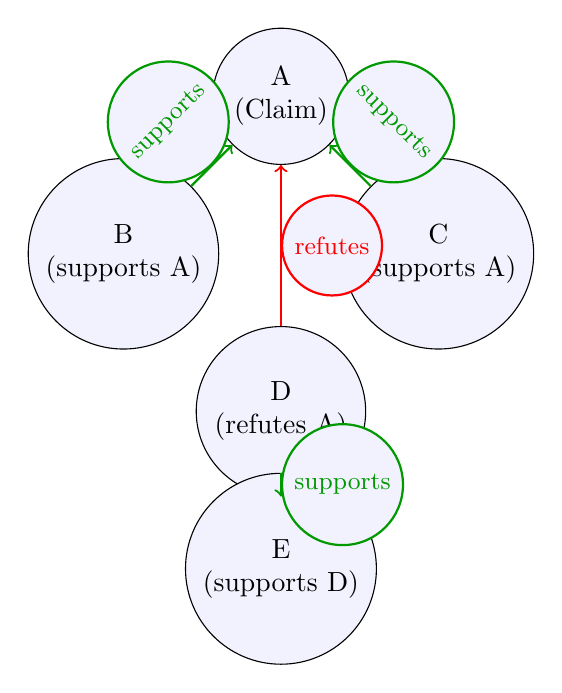
\begin{tikzpicture}[node distance=2.0cm and 2.5cm, every node/.style={draw, circle, fill=blue!5, minimum size=1cm, align=center}]
		\node (A) at (0,0) {A\\(Claim)};
		\node (B) at (-2,-2) {B\\(supports A)};
		\node (C) at (2,-2) {C\\(supports A)};
		\node (D) at (0,-4) {D\\(refutes A)};
		\node (E) at (0,-6) {E\\(supports D)};
		\draw[->, thick, green!60!black] (B) -- (A) node[midway, above, sloped]{\small supports};
		\draw[->, thick, green!60!black] (C) -- (A) node[midway, above, sloped]{\small supports};
		\draw[->, thick, red] (D) -- (A) node[midway, right]{\small refutes};
		\draw[->, thick, green!60!black] (E) -- (D) node[midway, right]{\small supports};
	\end{tikzpicture}
	\caption{Example evidence graph fragment. Node A represents an initial claim. Nodes B and C provide supporting evidence for A (green arrows). Node D provides a refuting evidence against A (red arrow). Node E supports the findings of D (i.e., replicates D's refutation of A). In the ASB system, this network of support and refutation relationships would be used to compute fragility scores for each node.}
	\label{fig:graph}
\end{figure}

In ASB, every research publication (or scientific claim) is represented as a node in a directed graph. We call this the \textbf{evidence graph}. An edge from node $B$ to node $A$ indicates that publication $B$ has cited publication $A$. However, unlike traditional citation indexes that do not distinguish the nature of the citation, ASB requires each citation to be annotated with its \emph{polarity}:
\begin{itemize}
	\item \textbf{Support}: If $B$'s findings \textit{support}, reproduce, or are consistent with the claims of $A$.
	\item \textbf{Refute}: If $B$'s findings \textit{contradict}, falsify, or cast serious doubt on the claims of $A$.
\end{itemize}
Each node can thus accumulate incoming links of either type over time as new papers cite it. These links form chains of evidence: for example, a paper $C$ might support paper $B$ which in turn refuted paper $A$, creating a sequence of evidence relationships.

Figure~\ref{fig:graph} illustrates a fragment of such an evidence graph. Each link is labeled as supporting (green arrow) or refuting (red arrow) evidence. This structure encodes not just which papers are connected, but the \emph{stance} of that connection, which is crucial for assessing credibility. A paper with many independent supporting replications will look very different in this graph from one that has attracted a well-substantiated refutation.

Importantly, this evidence graph is intended to be \textbf{open and evolving}. Anyone can add a new node (publish a new result) that cites prior work with appropriate support/refute designations. There is no central authority deciding which evidence is allowed; instead, the network grows organically as knowledge progresses. The graph provides a living documentation of the state of scientific testing for each claim. As evidence accumulates, the structure of the graph tells the story of how that claim has stood up (or faltered) under scrutiny.



\subsection{Evidence Fragility Score (EFS) algorithm}
The Evidence Fragility Score (EFS) is calculated by a trustless and recursive algorithm designed to evaluate the strength, transparency, and falsifiability of a research object without relying on consensus, reputation, or human authority.

EFS operationalizes the principle that textbf{falsifications are more epistemically significant than confirmations}. For example, if a claim $A$ has, say, five papers supporting it and no refutations, its ASB might be moderately high. But if a sixth paper comes along and refutes $A$ with strong evidence, that single refutation could outweigh the five supports, dramatically lowering $A$'s score. The refuting paper itself would receive a high score for providing compelling negative evidence. In effect, the system is constantly asking: "Has this claim been robustly challenged, and if so, did it withstand the test?" A claim that continues to be supported and never strongly refuted will see its score rise over time, whereas a claim that is refuted (or whose supporting evidence is undermined by later findings) will see its score fall.

Moreover, the \textbf{graph structure and the recursive nature of the EFS algorithm allows for the propagation of impact}. If a research $A$ is refuted by $D$, not only is $A$'s score reduced, but any other research $B$ that heavily relied on $A$ (say $B$ supported $A$ or built upon $A$'s result) may also suffer a hit to its EFS score, because one of the pillars supporting $B$ has cracked. EFS can capture this by dynamically recomputing scores so that the repercussions of new evidence ripple through the network. Over time, this helps prevent entire lines of research from resting on a faulty result: the moment the result is invalidated, the dependent work is flagged (via lowered scores) unless it can stand independently. 

\subsubsection{How It Works}
Each Research object carries metadata fields that describe its transparency, exposure to adversarial testing, funding conditions, and epistemic risk. 

The EFS algorithm combines the following key factors:
\begin{itemize}
	\item A local validation score - relates to Popper's falsifiability concept
	\item An antifragile funding score - relates to Taleb's \emph{skin in the game} concept and also the \emph{agent-principal problem}.
	\item An antifragile ruin score - to take into account the cost of being wrong.
	\item Recursive analysis of all linked research replications and refutations.
\end{itemize}

\subsubsection{Research Object Fields}
\begin{description}
	\item[\texttt{ruin\_scale}] Enum: \texttt{low}, \texttt{medium}, \texttt{high}. Used to calculate the ruin score dynamically.
	\item[\texttt{ruin\_impact}] Enum: \texttt{low}, \texttt{medium}, \texttt{high}. Used to calculate the ruin score dynamically.
	\item[\texttt{funders}] Array of objects. Each funder includes:
	\begin{itemize}
		\item \texttt{wallet\_id}: String. The identifier of the wallet.
		\item \texttt{anon}: Boolean. Whether the wallet is anonymous.
		\item \texttt{wallet\_age}: Integer. Wallet age in days.
		\item \texttt{amount}: Float. Amount funded.
	\end{itemize}
	\item[\texttt{data\_openness}] Enum: \texttt{none}, \texttt{partial}, \texttt{full}. Indicates the level of access to raw data and methods.
	\item[\texttt{validation\_enabled}] Boolean. Whether the research exposes raw data, methods, and test logic.
	\item[\texttt{test\_vectors}] Boolean. Whether test inputs and expected outputs are provided.
	\item[\texttt{refutations}] Count of formal, timestamped refutations logged on-chain.
	\item[\texttt{replications}] Count of successful replications with hash-verified results.
	\item[\texttt{research\_file\_url}] String. URL of the main research paper.
	\item[\texttt{research\_file\_hash}] String. Cryptographic hash of the research paper.
	\item[\texttt{data\_files}] Array of objects. Each object includes:
	\begin{itemize}
		\item \texttt{url}: String. URL where a dataset is stored.
		\item \texttt{hash}: String. Hash of the dataset to ensure integrity.
	\end{itemize}
\end{description}


\subsubsection{Validation Score}
\[
\text{validation}(R) = \mathbf{1}_{\text{validation\_enabled}} \cdot 0.4 + \text{data\_openness\_score} + \mathbf{1}_{\text{test\_vectors}} \cdot 0.2 + \log_2(n_{\text{rep}} + 1) \cdot 0.05 - n_{\text{ref}}
\cdot 0.1
\]

\subsubsection{Antifragile Funding Score}

Let $R$ contain a set of funders $F = \{f_1, f_2, \dots, f_n\}$, where each funder $f_i$ is a tuple $(\text{anon}_i, \text{wallet\_age}_i, \text{amount}_i)$. Then the funding score is computed as the
weighted average over all funders:

\[
\text{funding}(R) = \frac{\sum_{i=1}^{n} \text{amount}_i \cdot \left(1 - 0.2 \cdot \text{anon}_i - 0.1 \cdot \mathbf{1}_{\text{wallet\_age}_i < 30}\right)}{\sum_{i=1}^{n} \text{amount}_i}
\]

\subsubsection{Antifragile Ruin Score}
Let $\texttt{ruin\_scale}, \texttt{ruin\_impact} \in \{\texttt{low}, \texttt{medium}, \texttt{high}\}$. The final ruin score is computed as:

\[
\text{ruin}(R) = 1.0 + 0.25 \cdot \text{scale}(\texttt{ruin\_scale}) + 0.25 \cdot \text{impact}(\texttt{ruin\_impact})
\]

Where:
\begin{itemize}
	\item $\text{scale}(\texttt{low}) = 0$, $\texttt{medium} = 1$, $\texttt{high} = 2$
	\item $\text{impact}(\texttt{low}) = 0$, $\texttt{medium} = 1$, $\texttt{high} = 2$
\end{itemize}

This results in $\text{ruin}(R) \in [1.0, 2.0]$.

\subsubsection{The EFS Algorithm}
Let $R$ be a Research object. Then:
\[
\text{EFS}(R) =
\begin{cases}
	0 & \text{if } \text{isValid}(R) = \text{false} \\
	\frac{\text{validation}(R) \cdot \text{funding}(R)}{\text{ruin}(R)} + \sum_{i=1}^{m} \mathbf{1}_{\text{isValid}(R_i^{(\text{rep})})} \cdot \log_2(\text{EFS}(R_i^{(\text{rep})}) + 1) \cdot w_{\text{rep}}
	\\ - \sum_{j=1}^{n} \mathbf{1}_{\text{isValid}(R_j^{(\text{ref})})} \cdot \text{EFS}(R_j^{(\text{ref})}) \cdot w_{\text{ref}} & \text{otherwise}
\end{cases}
\]

Where:
\begin{itemize}
	\item $w_{\text{rep}}$: weight per replication (e.g., $0.05$)
	\item $w_{\text{ref}}$: weight per refutation (e.g., $0.1$)
\end{itemize}


\section{Conclusion}
The Antifragile Science Blockchain platform represents a paradigm shift in how we evaluate and incentivize scientific knowledge. Instead of relying on human consensus or pre-existing reputations, ASB grounds credibility in the objective relationships of support and refutation documented across studies. We have discussed how this approach is deeply rooted in the philosophy of science: it embodies Popper's falsifiability criterion by structurally rewarding refutation, and it echoes Taleb's insights by making the system antifragile and requiring genuine stakes (skin in the game) for scientific claims. 

By contrast, consensus-driven and authority-driven models can too easily conflate popularity with truth. ASB breaks that link, ensuring that even a lone dissenting experiment can carry the day if it is backed by decisive evidence. In doing so, it preserves the core scientific virtue of skepticism and continuous testing. The open, decentralized nature of the protocol further ensures that no viewpoint can be unfairly censored and that the system as a whole learns from its errors over time.

Implementing ASB in practice would mark a significant step toward a more resilient and trustworthy scientific ecosystem. It aligns incentives for researchers to pursue rigorous replication and bold falsification, knowing that both contribute to the credibility calculus. It provides consumers of scientific information (whether other researchers, policymakers, or the public) with a more informative metric than citation counts or journal names—a metric that reflects how battle-tested a given result is in the arena of evidence.

In summary, \textbf{truth without consensus} is not only a philosophical stance but a practical design principle for scientific knowledge systems. The ASB protocol operationalizes this principle, offering a blueprint for a self-correcting, evidence-first approach to evaluating truth. In a world increasingly awash with data and claims, such a protocol could serve as a much-needed compass, always pointing back to the solid ground of empirical evidence as the final arbiter of credibility.

\bibliographystyle{plain}

\bibliography{bibs/Popper1963,bibs/Taleb2012,bibs/Taleb2018,bibs/CBSnewsPurduePharma,bibs/PBSPurduePharma,bibs/Alonso2021,bibs/GLENNA2021104290,bibs/mindthegap2020,bibs/ehn2018,bibs/USvsHolmes2022,bibs/buzzfeednews2018,bibs/justivegove-theranos,bibs/Semmelweis2006,bibs/WGMcbride,bibs/Diethylstilbestrol2000,bibs/Wolff1997,bibs/Fitzpatrick2006,bibs/VarleyVarma2021}

\end{document}

